\documentclass{article}

\usepackage[left=3cm, right=3cm]{geometry}

\usepackage{minted}
\usepackage{dirtree}
\usepackage{graphicx}
\usepackage{float}

\setlength{\parindent}{0pt}

\begin{document}

\title{NameSayer User Manual}
\author{Jordan Sim-Smith \\
		The University of Auckland \\
		\and
		Joshua Fu \\
		The University of Auckland \\
		}

\maketitle

\clearpage

\tableofcontents

\clearpage

\section*{Target User}
NameSayer's target user is the Dean of Engineering. The Dean will use this
application to practice students' names before the graduation ceremony.

\section{Setup}

This page describes the system requirements to run NameSayer, and will guide the
user through system setup and the launch of the NameSayer application.

\subsection{Required Software}

NameSayer has been designed to run on a Linux based Operating System, relying on
bash system calls. To run NameSayer, please ensure that you are running a Linux
distribution with a Graphical User Interface. \\

NameSayer also requires a \textbf{Java Runtime Environment} to run in and the
\textbf{ffmpeg} program used for audio manipulation. \\

Using a terminal, Java 8 can be installed as follows:
\begin{minted}{bash}
$ sudo add-apt-repository ppa:webupd8team/java
$ sudo apt update
$ sudo apt install oracle-java8-installer
\end{minted}

Similarly, ffmpeg can be installed as follows:
\begin{minted}{bash}
$ sudo apt update
$ sudo apt install ffmpeg
\end{minted}

\subsection{Required Hardware}
The NameSayer application involves the recording and playback of audio.
Therefore, NameSayer requires that the user's computer has either an internal or
external microphone that is turned on. The user should ensure that their
computer has audio playback capability (speakers) and that they are turned on.

\subsection{Launching NameSayer}
Before launching NameSayer, the names database must be placed in a folder called
\textbf{names} in the same directory as  the executable jar. \\

\dirtree{%
	.1 namesayer.
	.2 names.
	.2 namesayer.jar.
	.2 README.md.
	.2 user-manual.pdf.
} \ \\

NameSayer must be run from the command line. The user must first navigate into
the NameSayer folder. Then the application can be launched as follows:

\begin{minted}{bash}
$ java -jar namesayer.jar
\end{minted}

\section{Home Screen}

\begin{figure}[H]
	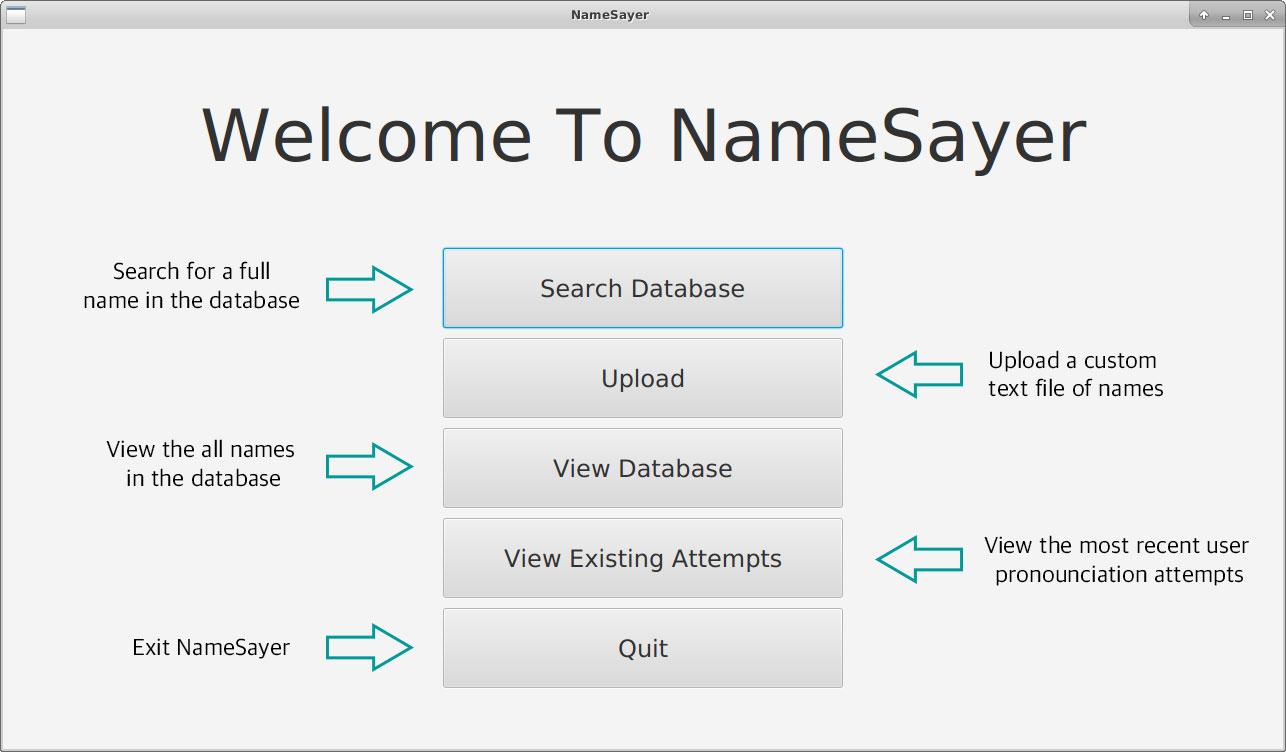
\includegraphics[width=\textwidth]{images/1_home.jpg}
	\caption{The home screen of NameSayer.}
	\label{home}
\end{figure}

\section{View the Database}
The Database View allows the user to view all the names that are  featured in
the current name database. Composite names can be constructed from base names
and added to a playlist. This playlist can then be practised in the practice
screen.

\subsection{Viewing Features}
The list of names on the left of the screen allow users to quickly browse
through all available names in the database. The list is in alphabetical order
for user convenience. \\

The list of names on the right side of the screen contains the list of names
that the user has chosen to practice. \\

The centre of the screen shows the result of the name currently being built.
This name will change accordingly as users select and  deselect names from the
database.

\subsection{Usage Instructions}

\begin{enumerate}
	\item Construct full names by selecting the checkboxes next to each part of
	the name in order.

	\item The name currently being built will appear in the centre of the
	screen.

	\item Users can add more names to the current name by repeating step 1 or
	remove particular parts by deselecting the checkboxes.

	\item Select \textbf{Add Name} to transfer the select names to the list
	under \textbf{Names to Practise}.

	\item Users can add more full names to the list by repeating steps 1-4.

	\item {\em Optional: } users can shuffle the playlist by selecting the
	\textbf{Shuffle} checkbox.

	\item Select the \textbf{Playback} button when ready. This will take the
	user to the practice screen where the constructed playlist can be practised.

\end{enumerate}

\begin{figure}[H]
	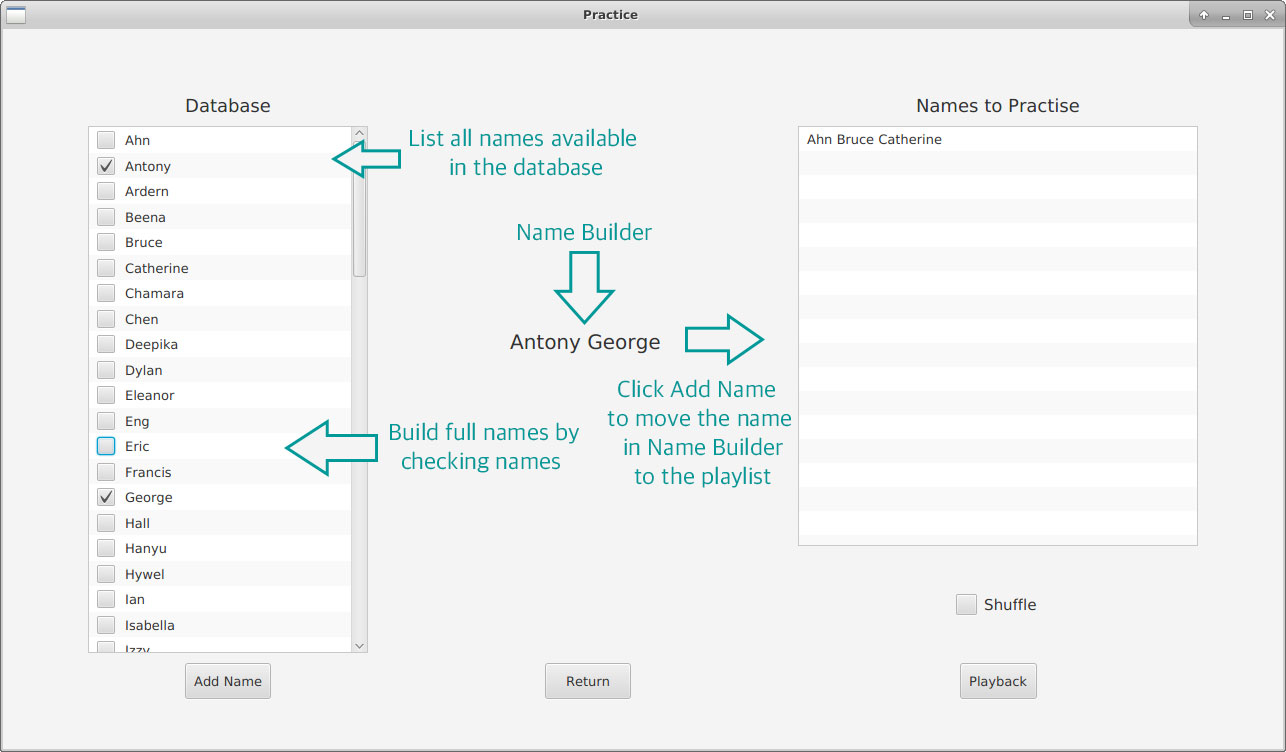
\includegraphics[width=\textwidth]{images/2_view_build.jpg}
	\caption{Building a name to practice on the view screen.}
	\label{viewbuild}
\end{figure}


\begin{figure}[H]
	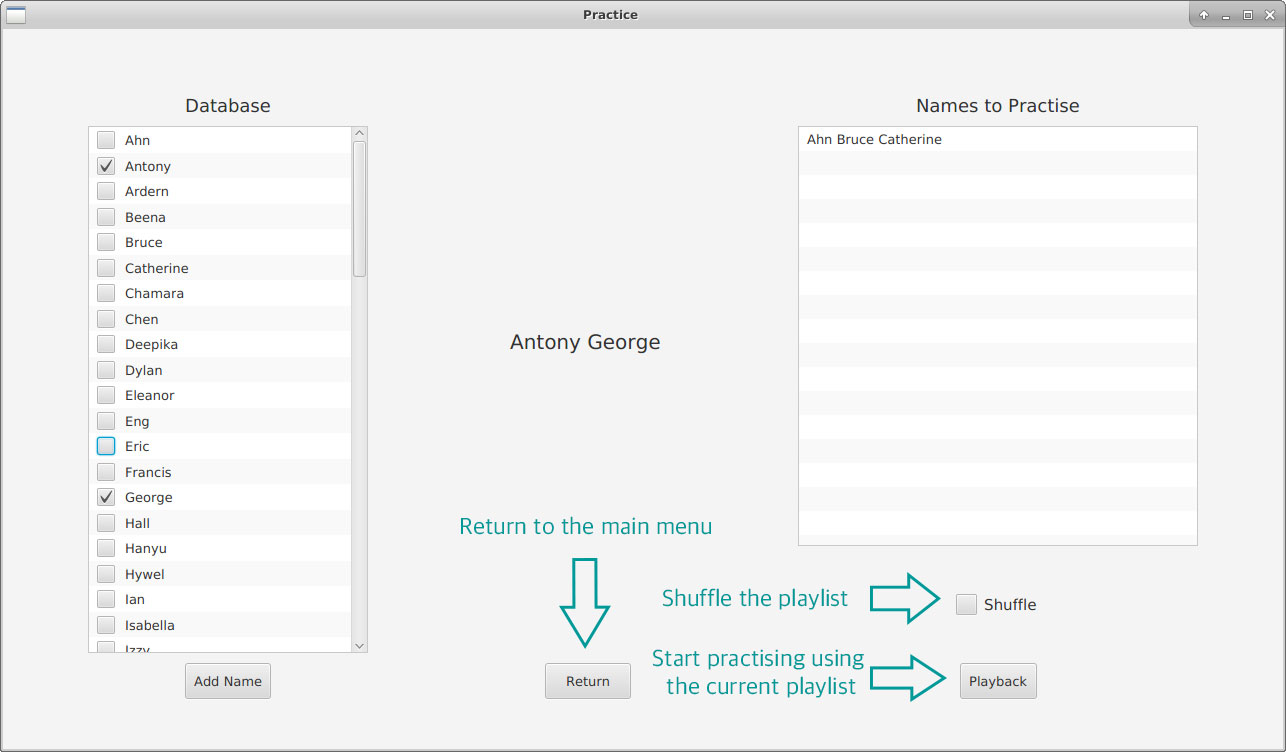
\includegraphics[width=\textwidth]{images/3_view_play.jpg}
	\caption{Practice the built playlist on the view screen.}
	\label{viewplay}
\end{figure}


\section{Search the Database}
The Search Screen allows a user to search for one or more names in the NameSayer
database. Using this feature, the user can request a specific name without
having to find it manually in the database. NameSayer will notify the user if
parts of the requested name are unavailable.

\subsection{Search Instructions}

\begin{enumerate}
	\item Search for the desired name or list of names using the textfield.

	\item Select the \textbf{Search} to process the search.

	\item The application will return a list of names found in the database and
	another list of names in red that represents names that are unavailable.

	\item The user can perform another search in the same way if they are
	unsatisified with the search results.

	\item Once satisfied with the search results, select the \textbf{Practice}
	button. This will take the user to the practice scene where the found names
	can be practised.

\end{enumerate}

\begin{figure}[H]
	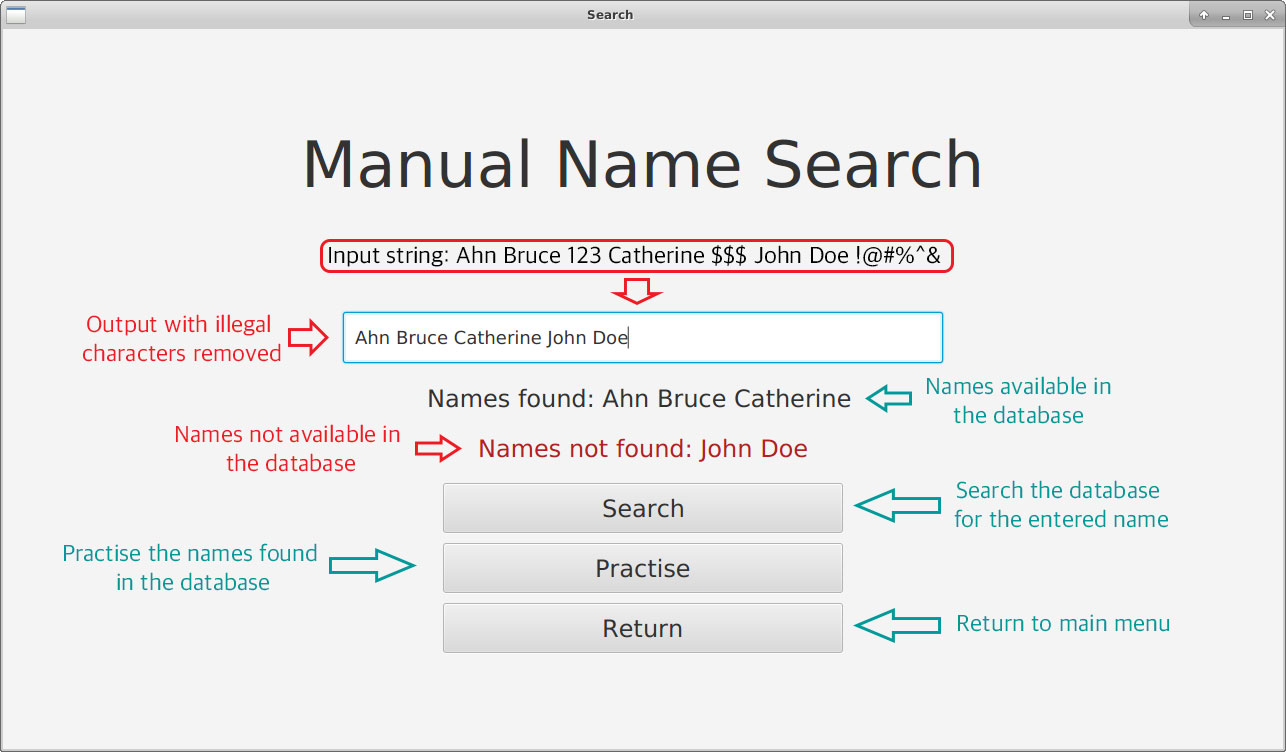
\includegraphics[width=\textwidth]{images/4_search.jpg}
	\caption{Searching for a name on the search screen.}
	\label{search}
\end{figure}

\section{Upload a Custom List}
The Upload screen allows a user to upload a custom list of names so that they
can be practised in NameSayer.  NameSayer will scan through the names in the
file, and create a play list of the names found. This playlist can then be taken
to the practice scene and be practised.

\subsection{Upload Instructions}

\begin{enumerate}
	\item Select the \textbf{Upload} button. NameSayer will prompt the user to
	select a text file. Please note, the file browser is set to show .txt files
	only.

	\item After selecting the desired file, NameSayer search for every entry in
	the file. Names available to be practised will be displayed in black and
	those unavailable in red.

	\item Users can then choose to upload further text files using the
	\textbf{Upload} button.

	\item Select the \textbf{Practise} button to start practising. This will
	take the user to the Practice screen.

\end{enumerate}

\subsection{File Format}
Files uploaded to NameSayer must be a plain text file (.txt format).  Multiple
names that are to be practised together should be on the  same line. These names
should be separated by either a space or a hyphen. Names that are to be
practised separately should be on different lines. \\

Here is an example of a correctly structured file.
\begin{minted}{bash}
Jami-Lee Ross
Jacinda Adern
David Seymour
John Key
\end{minted}

\begin{figure}[H]
	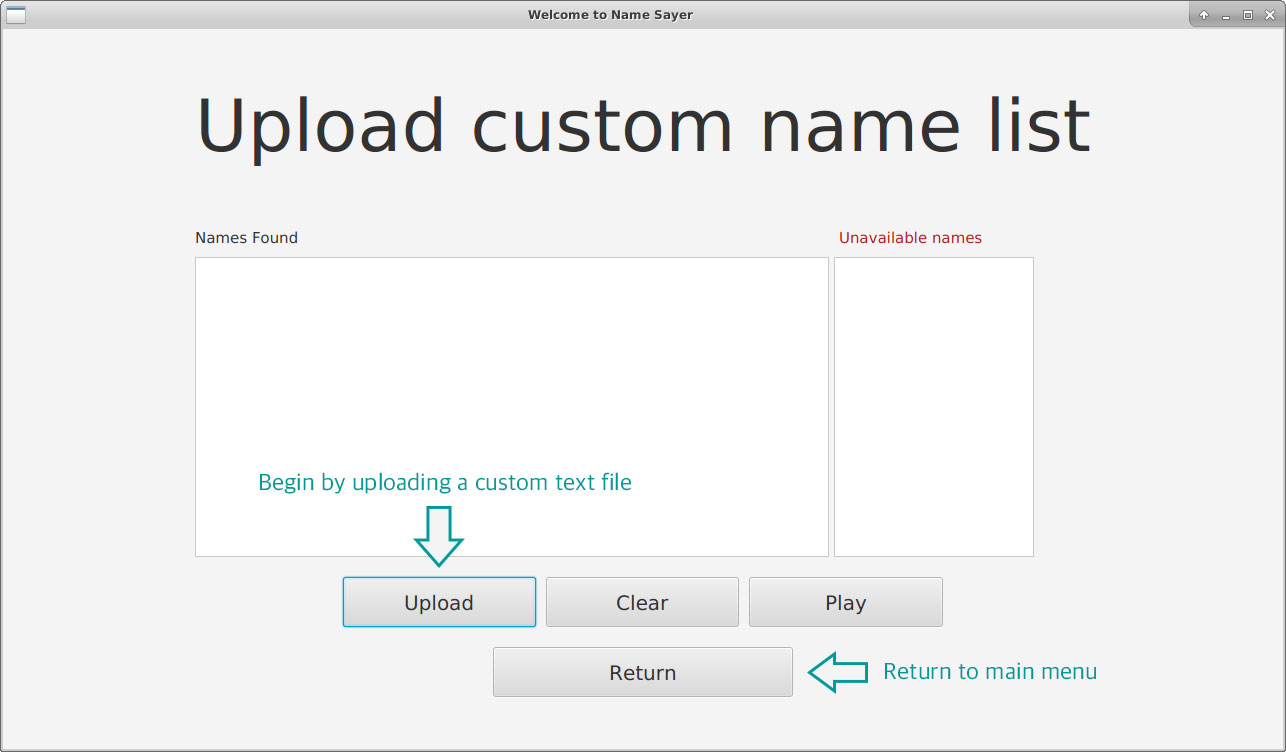
\includegraphics[width=\textwidth]{images/5_upload_empty.jpg}
	\caption{Uploading a custom text file of names.}
	\label{uploadempty}
\end{figure}

\begin{figure}[H]
	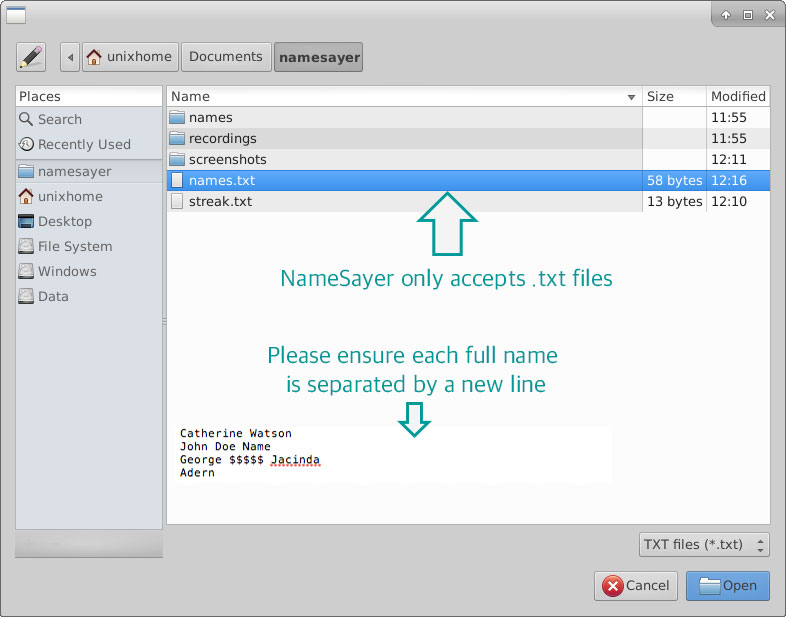
\includegraphics[width=\textwidth]{images/6_upload_filesystem.jpg}
	\caption{Searching for a .txt file to upload.}
	\label{uploadfilesystem}
\end{figure}

\begin{figure}[H]
	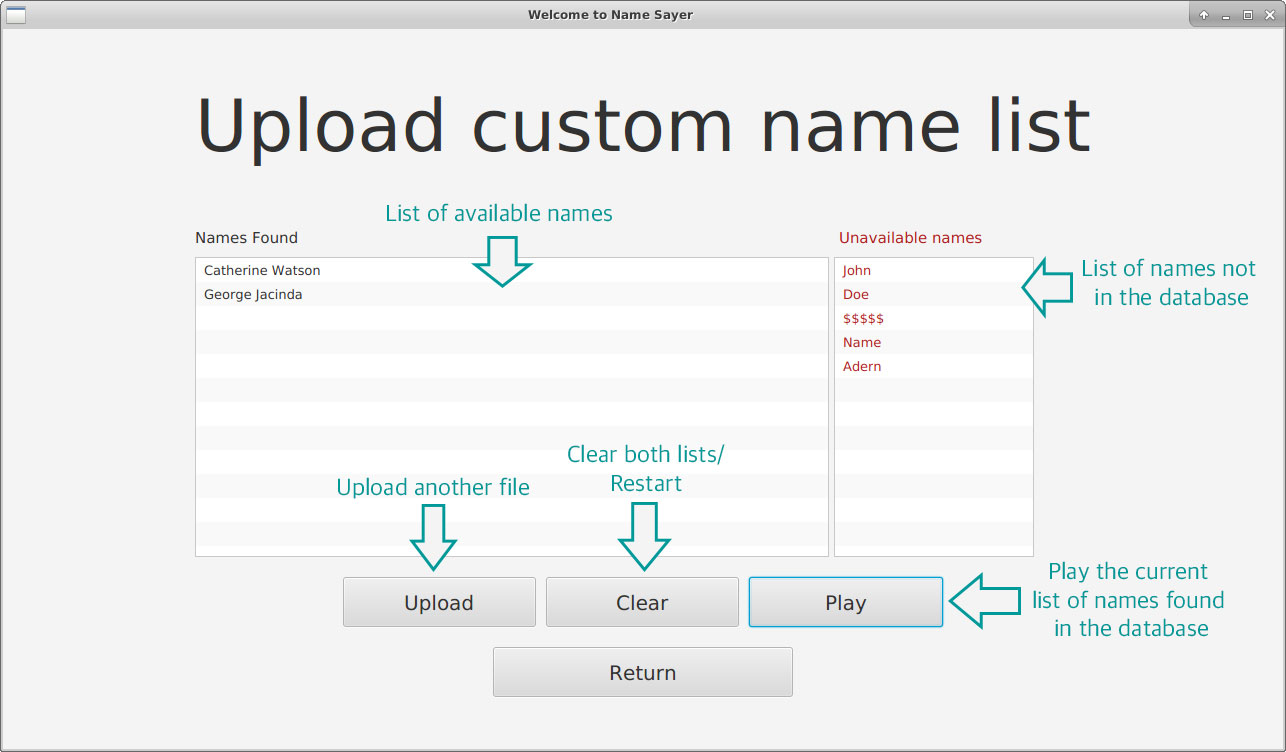
\includegraphics[width=\textwidth]{images/7_upload_populated.jpg}
	\caption{Playlist has been created from the uploaded file.}
	\label{uploadpopulated}
\end{figure}

\section{Name Practice}
The Practice screen is central to the application and most likely where the user
will spend the majority of their time. The practice scene allows the user to
hear, record and compare their attempts to selected names from the database. The
names available  in the practice screen are selected previously in the upload/
search or view screens.

\subsection{Basic Features}

\begin{itemize}
	\item \textbf{Name List} - shown on the left is the list of names to be
	practised in this current session. The names will be played in the order
	that  they are shown in this list. Entries in the Name List can either be an
	individual name or a group of names that are to  be practised together.
	Names are not selected to be practised from this list, the user should use
	the next and previous buttons instead.

	\item \textbf{Current Name} - shown largely in the centre of the page is the
	name that is currently being practised. The current name will update when
	the user progresses through the names in the Name List.

	\item \textbf{Play Button} - the play button, shown in the centre of the buttons
	at the bottom of the page is used to play the current name.

	\begin{itemize}
		\item If \textbf{Listen Only} is selected, then the current name will be played
		to the user, so that they can hear the sound without recording.

		\item If \textbf{Listen Only} is not selected, then the user will be
		taken through the recording process. Firstly, the name will be played
		outloud as before. Then the user will be prompted that the recording
		will start when they are ready. After recording, the original name
		followed by the user's attempt will be played for comparison. The user
		is then presented with the opportunity to save or to discard this
		attempt.

    	\item The progress bar located directly below the current name displays
    	information about the state of the recording process as well as
    	displaying how long the user has left to record their attempt.

	\end{itemize}

	\item \textbf{Navigation Buttons} - the previous and next buttons are used
	to navigate through the list of names that are being  practised. When a user
	is comfortable with practising the current name, they can use the next
	button to attempt the next name.  To return to a previous name, the user can
	use the previous button. A user can remain as long as desired on a name, and
	can  navigate through the name list at their own pace.

	\item \textbf{Return Button} - the return button, located in the bottom
	right of the screen, will end this practice session and will return the user
	to the home menu where they can perform other actions or exit the
	application.

\end{itemize}

\begin{figure}[H]
	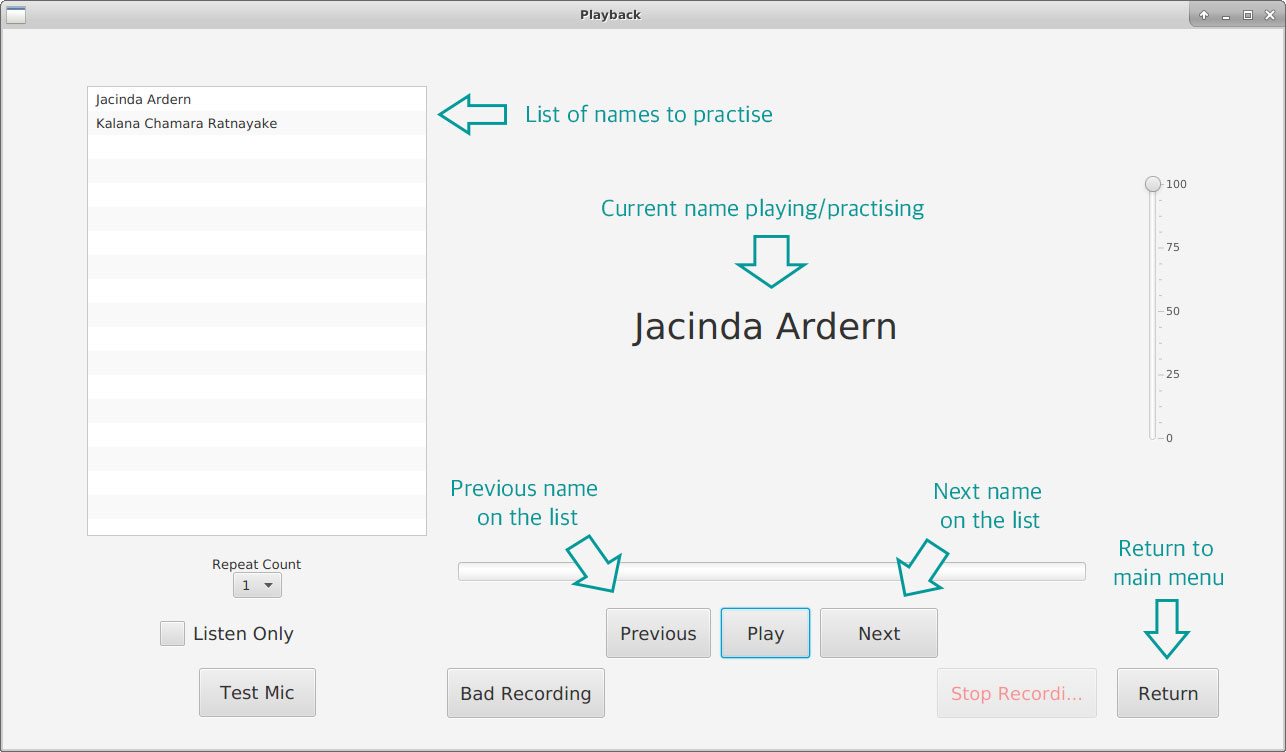
\includegraphics[width=\textwidth]{images/8_practice_nav.jpg}
	\caption{Basic features of the play screen.}
	\label{practicenav}
\end{figure}

\begin{figure}[H]
	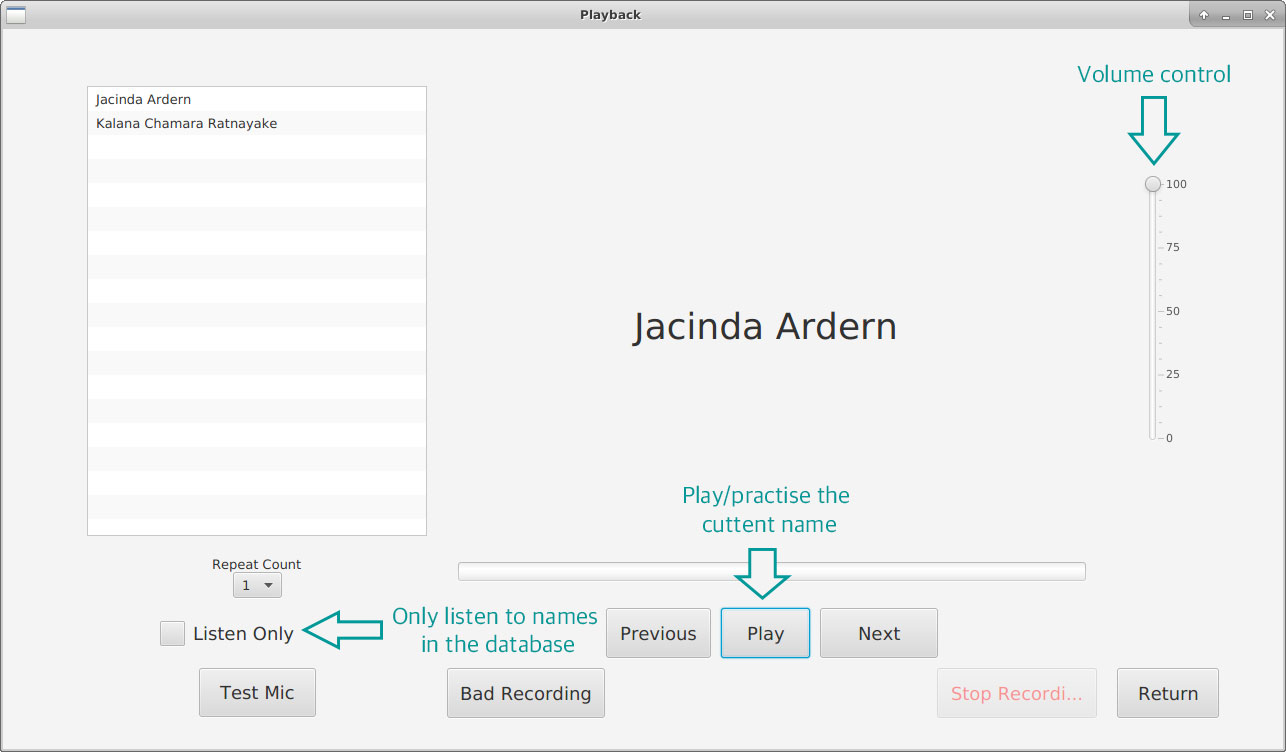
\includegraphics[width=\textwidth]{images/9_practice_play.jpg}
	\caption{Playing the current name from the play screen.}
	\label{practiceplay}
\end{figure}

\subsection{Advanced Features}

\begin{itemize}
	\item \textbf{Volume Slider} - the volume slider is located on the far right
	of the screen. The volume slider controls the volume at which the practised
	names are played back to the user. The slider ranges between 0 (muted) and
	100 (maximum volume). The default setting of the slider is 100. To adjust
	the playback audio, the user should move the slider knob to the desired
	value before playing a name.

	\item \textbf{Test Microphone} - the option for the user to test their
	microphone level is located in the bottom left corner of the screen. This
	button will cause a popup with a live detection of the volume level captured
	by the microphone. The higher the blue bar, the greater the volume captured
	by the microphone.

	\item \textbf{Bad Recording} - when practising names from the database, the
	user may encounter names of poor quality. To flag this name to  the database
	administrator, the user can select the bad recording button. This button
	will prompt the user to select which of the  individual names was of bad
	quality, catering for several names being played together. Furthermore,
	badly rated names are will not  be played when there are names of better
	quality present.

	\item \textbf{Stop Recording} - if the user has finished recording their
	attempt in less than the 5 seconds provided, they can select the stop
	recording button displayed in red. This button will skip over the remaining
	recording time and proceed to comparing the  attempt against the original.
	The user should take care not to press this button before finishing their
	attempt, as it will not record anything after it is pressed.

	\item \textbf{Repeat Count} - the repeat count dropdown selection is located
	on the left side of the screen. This option determines  how many times the
	comparison between the user recording and the database recording will be
	played. The default value is 1,  however the user can choose for the
	comparison to be looped over up to 5 times.

\end{itemize}

\begin{figure}[H]
	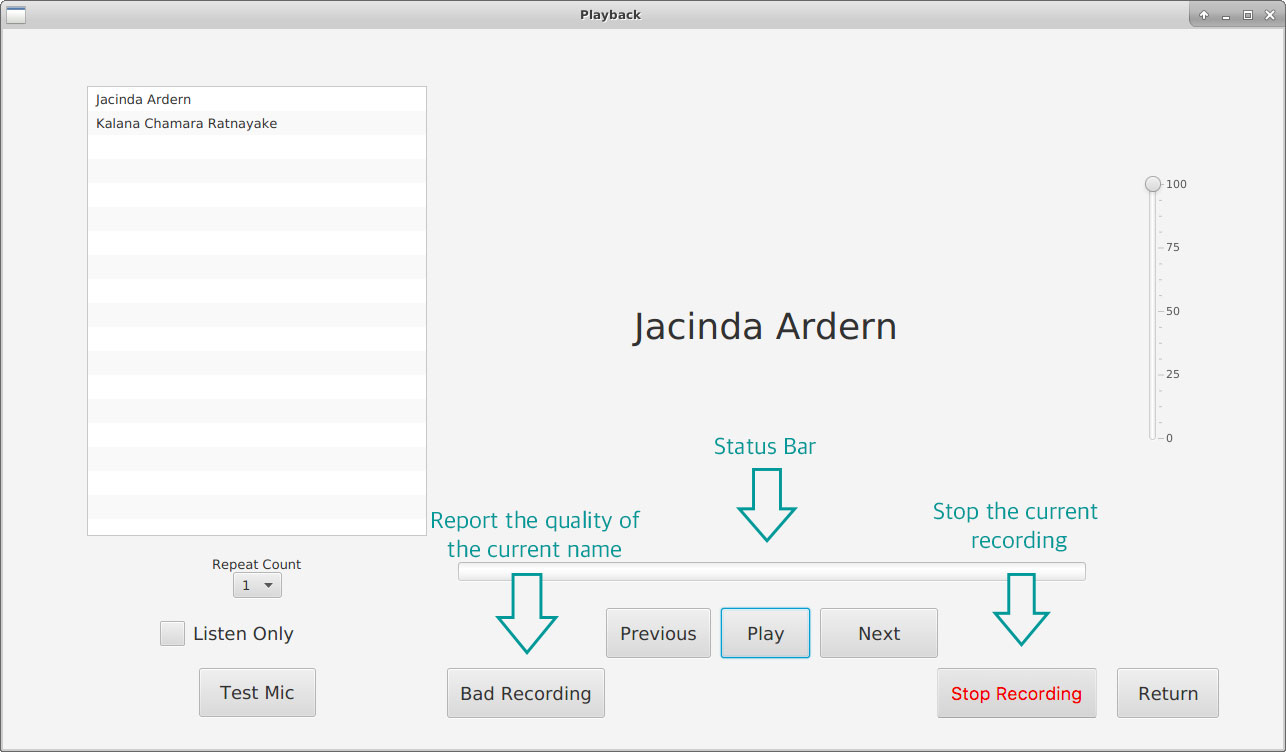
\includegraphics[width=\textwidth]{images/10_practice_adv.jpg}
	\caption{Advanced features of the play screen.}
	\label{practiceadv}
\end{figure}

\begin{figure}[H]
	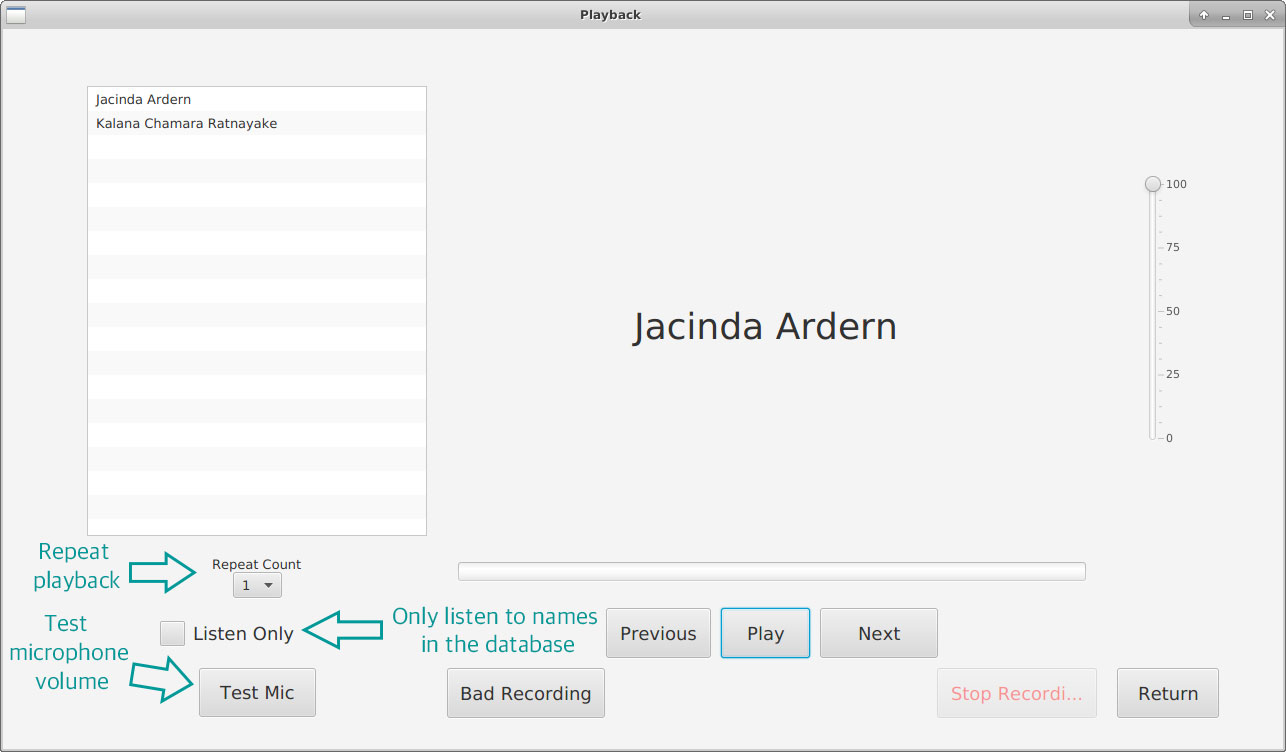
\includegraphics[width=\textwidth]{images/12_practice_config.jpg}
	\caption{Configuration for the play screen.}
	\label{practiceconfig}
\end{figure}

\section{View Past Attempts}

Each time a user records an attempt for a name or group of names, they are
presented with an option to save that attempt. The last attempt for each name
combination will be saved, i.e. new saved attempts from the user will overwrite
the existing saved attempt. Historical user attempts can be accessed from the
main menu by selecting the \textbf{View Existing Attempts} button. \\

The Existing attempts screen is fairly simple. In the middle of the screen, the
list of available user attempts are displayed in alphabetical order for the
user's convenience. Each entry to this list contains the name or names that was
practised and recorded, and the date that it was recorded on. An example entry
would be {\em James Jacinda - Wed Jan 03 21:07:21 NZDT 2018}. In this case, the
names practiced were James and Jacinda, in that order, and the date that it was
practised on was Wednesday the 3rd of January. \\

Below the list of saved attempts is a simple volume slider. This volume slider
allows the user to adjust the volume that the  recordings are played back. The
values on the slider range from 0 (muted) to 100 (maximum volume). The default
value is 100. To use the  volume slider, the user needs to simply adjust the
volume before selecting a recording attempt to play. \\

Below the volume slider is the play button. The play button is used to hear the
past user recording for the attempt selected in the list. To use the play
button, the user should first select the recording that they would like to hear,
and then press the play button. If no recording is selected, then a warning
dialogue will pop up, guiding the user into selecting a recording  before
playing. \\

Finally, the close button at the base of the screen is used to close this screen
and return to the main menu.

\begin{figure}[H]
	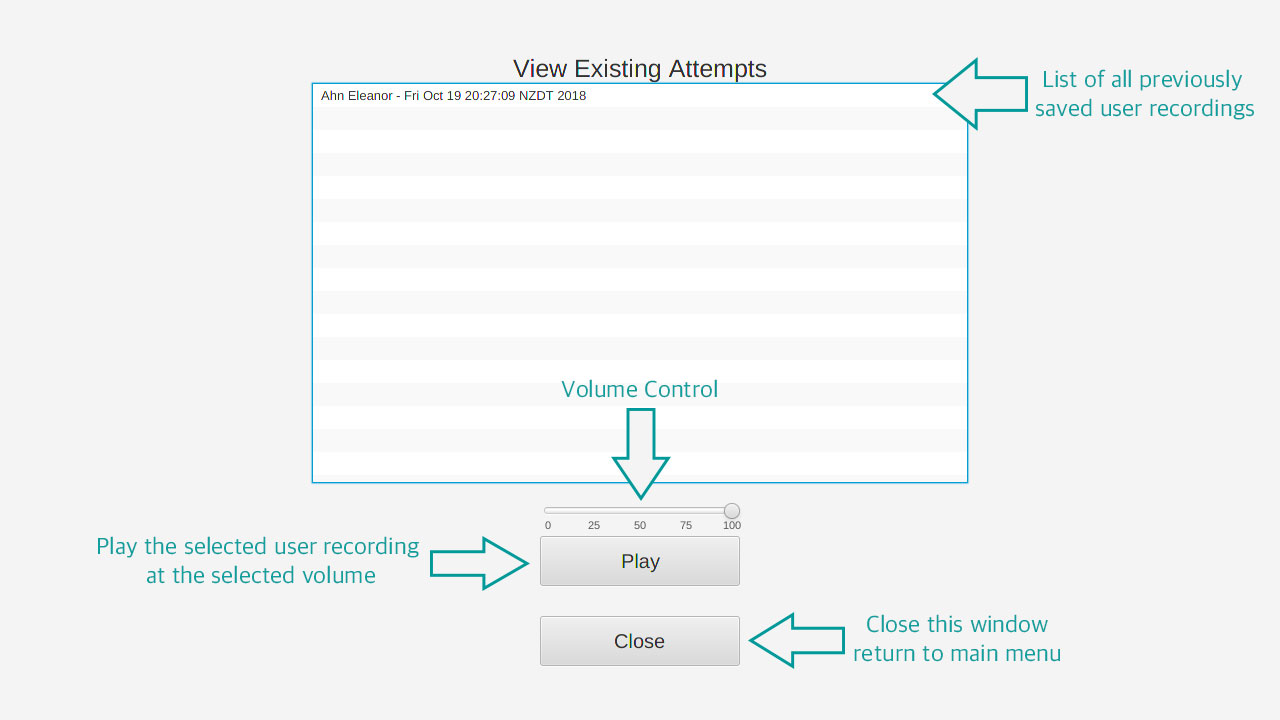
\includegraphics[width=\textwidth]{images/16_existing-attempts.jpg}
	\caption{Viewing existing attempts.}
	\label{existingattempts}
\end{figure}

\section{Special Features}
To enhance the user's experience with NameSayer, several special features have
been added. These features have been designed with both the target user and all
other users in mind.

\subsection{Streaks}
A NameSayer streak occurs when the user has been using the program for at least
2 days consecutively. Every consecutive day  that a user uses NameSayer, the
streak will be incremented. If a user does not log onto NameSayer for a whole
day, the  streak will be reset. Streaks are an effective form of motivation for
the user to keep returning to the application,  improving their name
pronunciation. \\

Upon opening the NameSayer application, if a streak is present, the user will be
congratulated on their consistent efforts. A pop up window will appear, with an
affirmation as well as the length of the streak (number of days).

\begin{figure}[H]
	\centerline{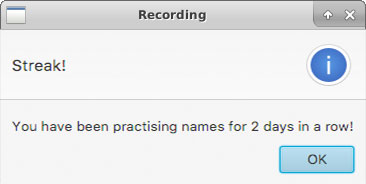
\includegraphics[width=\textwidth/2]{images/15_streak.jpg}}
	\caption{Streak pop up upon NameSayer launch.}
	\label{streak}
\end{figure}

\subsection{Selective Rating}
NameSayer offers the option to either practice a name individually or amongst a
group of other names, for example, practising a persons's first and last name
together. Upon listening to a name in the database of low quality, the user may
choose to flag this name to the database maintainer using the \textbf{Bad
Recording} button. \\

When practising more than one name at once, the user may require that one or
more of the played names be flagged as low quality. The \textbf{Bad Recording}
button prompts the user to select the name that they would like to flag, instead
of flagging the whole selection or none of it.

\begin{figure}[H]
	\centerline{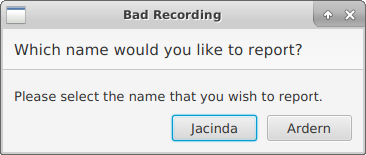
\includegraphics[width=\textwidth/2]{images/11_bad_recording.png}}
	\caption{Selecting which name to rate.}
	\label{badrecording}
\end{figure}

\subsection{Multiple File Upload}
One of the features of NameSayer is that a user can upload a text file
containing a list of names to be practised together or  sequentially. NameSayer
extends this functionality such that multiple lists can be combined together,
instead of restricting the user to a single file upload.

\subsection{Live Search Validation}
Another feature of NameSayer is an explicit search for a name or group of names.
To enhance usability, NameSayer filters  the user's search query in real time
for invalid characters. Thus, the user's search will not be invalidated because
of disallowed characters. A live filter is also much more intuitive for the
user. Instead of typing out an entire query to be told that it is invalid, a
live filter lets a user know right away what can be searched for and what can't
be.

\end{document}
